\documentclass[11pt,letterpaper]{article}
\bibliographystyle{ieeetr}
\usepackage[backend=biber,style=numeric]{biblatex} 
\addbibresource{reference.bib} 
\usepackage[utf8]{inputenc}
\usepackage{graphicx}

\usepackage{fullpage}

\begin{document}


\title{Knowledge-CLIP for Limited Data: Enhancing Semantic Alignment in Small-Scale Datasets}


\author{
Zhanhao Liu (zhanhaol@umich.edu), 
Huanchen Jia (jhuanch@umich.edu),\\
Qiulin Fan (rynnefan@umich.edu),
Lingyu Meng (jmly@umich.edu)
}

\date{02/03/2025}


\maketitle


\section{Problem statement}
Multimodal representation learning, particularly through frameworks like Contrastive Language–Image Pretraining (CLIP), has shown significant promise in bridging the gap between textual and visual data. CLIP-based models excel in tasks such as zero-shot classification, cross-modal retrieval, and transfer learning by learning joint embeddings of text and images. However, the performance of these models is heavily reliant on the quality, diversity, and scale of the training data. Current multimodal datasets often suffer from issues such as biases, noise, imbalances, and limited diversity, which can hinder the generalization and robustness of CLIP-based systems. While much attention has been given to improving model architectures and training strategies, there is a critical need to explore data-centric methods—such as dataset curation, augmentation, debiasing, and sampling—to address these challenges. This research focuses on developing and evaluating data-centric approaches to enhance the effectiveness of CLIP-based multimodal representation learning, ultimately enabling more reliable and scalable models for real-world applications.\\
We aim to design data-centric augmentations to improve CLIP performance on small training datasets. Our current interest lies in adpting and improving the Knowledge-CLIP framework\cite{pan2022contrastivelanguageimagepretrainingknowledge} to small-sized datasets, and further create our own model based on it.



\section{Significance}
Contrastive Language–Image Pretraining (CLIP) has revolutionized multimodal representation learning by enabling models to learn joint embeddings of text and images through contrastive learning. While CLIP has shown remarkable performance in zero-shot and transfer learning tasks, its effectiveness is highly dependent on the quality, diversity, and scale of the training data. Existing multimodal datasets often contain biases, noise, and imbalances, which can hinder the generalization and robustness of CLIP-based models. Despite significant progress in model architectures and pretraining strategies, the role of data-centric methods—such as dataset curation, augmentation, debiasing, and sampling—remains underexplored. Addressing these data-related challenges is critical to unlocking the full potential of CLIP-based multimodal representation learning.



\section{Related work}
\subsection{Existing Methods:}
CLIP (Contrastive Language-Image Pre-Training) is a multimodal representation learning model which leanrs to understand both text and image jointly by combining them in a shared embedding space. And its performance is shown recently that it could be enhanced by leverging the difficulty in training.\\
Currently the exisiting methods mostly improve in the following perspectives.\\
\begin{itemize}
    \item \textbf{Hard Negative Mining}: Hard negative examples are those that are semantically similar to the positive samples but belong to different classes, making it challenging for the model to distinguish between them. In contrastive learning, two primary strategies enhance model performance: generation-based methods and regularization-based methods. Generation-based methods, such as NegCLIP and SVLC, create hard negatives by altering positive samples to produce semantically similar yet incorrect pairs, challenging models to discern subtle differences. Regularization-based methods employ strategies like intra-modal contrastive loss and ranking cross-modal hard negatives to refine learning.
    \item \textbf{Fine-Grained Cross-Modal Alignment Fine-Tuning}: Some previous works such as FILIP enhances multimodal alignment by matching local image patches with specific text tokens via a similarity matrix. Unlike CLIP’s global image-text matching, it computes token-level contrastive losses, forcing visual and textual tokens to mutually select their most relevant counterparts. The regional information and details could be better learned this way.
    \item \textbf{Rewrite Empowered by Large Language Model}: LaCLIP generates diverse text rewrites for each image caption via LLMs while preserving semantic meaning, boosting the performances significantly on datsets such as  CC12M and LAION-400M . 
\end{itemize}
\subsection{Comparisons:}
DeCLIP combines the idea of \textbf{Hard Negative Mining} and \textbf{Fine-Grained Cross-Modal Alignment Fine-Tuning} such that the model can deepen its understanding of the entire image by paying attention to the regional changes of the image. From the proposed method section, DeCLIP uses Large language model to capture keywords from the caption in the data set and replaces those keywords one at a time with pre-trained catogeries, forming our final traning set. It is different from \textbf{Hard Negative Mining} in applying the changes to \textbf{images} instead of \textbf{texts}, while it is improved based on \textbf{Fine-Grained Cross-Modal Alignment Fine-Tuning} by considering contexts of texts and layout of images
\subsection{Core Model and Tool References:}
Our framework integrates multiple state-of-the-art tools for multimodal tasks. The core part is CLIP itself combining text and image processing.
For \textbf{text extractions}, we utilize the \texttt{spaCy} library with its small English language model (\texttt{en\_core\_web\_sm}), which takes out nouns effecitvely and merge compound noun if needed. 
Mapping from extracted nouns to pre trained catogories is captured using the \texttt{word2vec-google-news-300} embeddings, a 300-dimensional model trained on 3 billion words from Google News. 
For \textbf{images segmentation}, we deploy \texttt{yolov8n-seg.pt}, a lightweight variant of YOLOv8-seg pretrained on COCO, and optimize inference via ONNX export. Smoothing of the images is enhanced by integrating \texttt{CLIP} through the \texttt{runwayml/stable-diffusion-inpainting} pipeline, enabling robust image-text understanding in tasks like inpainting.
\section{Proposed Approach}
Knowledge-CLIP enhances CLIP's performance in semantic alignment and reasoning tasks by incorporating Knowledge Graphs (KGs), which enable the extraction of structural information between entities. Additionally, it leverages Knowledge Distillation (KD) Loss to distill knowledge from the original CLIP model, preventing catastrophic forgetting when adapting to new tasks.

Originally, Knowledge-CLIP was designed for large-scale datasets and heavily relies on a multimodal transformer architecture. However, we argue that its knowledge-driven semantic alignment capability can be effectively adapted to small-scale datasets. The \textbf{KG-enhanced learning} mechanism in Knowledge-CLIP provides several advantages:
\begin{itemize}
    \item Compensating for missing relational information in small datasets, mitigating the risk of overfitting to a limited data distribution.
    \item Improving the model’s ability to understand object attributes and relationships, thereby enhancing generalization.
\end{itemize}
Our goal is to modify Knowledge-CLIP to ensure its effectiveness on small datasets while retaining its knowledge-enhanced learning capabilities. Specifically, at this time as a draft, we plan to:
\begin{enumerate}
    \item Retain Knowledge-CLIP’s knowledge enhancement mechanism while\textbf{ removing its complex multimodal transformer structure} to reduce computational overhead.
    \item \textbf{Replace the heavy encoders with lightweight alternatives}:
    \begin{itemize}
        \item Image encoder: Replace ViT-Large with ViT-Small.
        \item Text encoder: Replace CLIP’s Transformer with \textbf{DistilBERT} or other lightweight models.
    \end{itemize}
    \item Incorporate more efficient optimization strategies, such as \textbf{SimCLIP}\cite{liu2024an} and \textbf{Adaptive Hard Negative Mining (AHNM)}, introducing a more lightweight contrastive learning optimization strategy.
    \item Freeze part of the model parameters, fine-tuning only the \textbf{top layers and projection head}, reducing overfitting risks associated with small datasets.
    \item Apply\textbf{ Low-Rank Adaptation (LoRA)} within Knowledge-CLIP’s multimodal module, adapting only a small subset of parameters for efficient training.
    \item \textbf{Introduce Fair Contrastive Loss (FCL)\cite{alabdulmohsin2024clipbiasusefulbalancing}} to prevent the model from learning spurious associations present in the dataset, thereby reducing Representation Bias.
\end{enumerate}

\subsection{Pipeline illustration}
\begin{center}
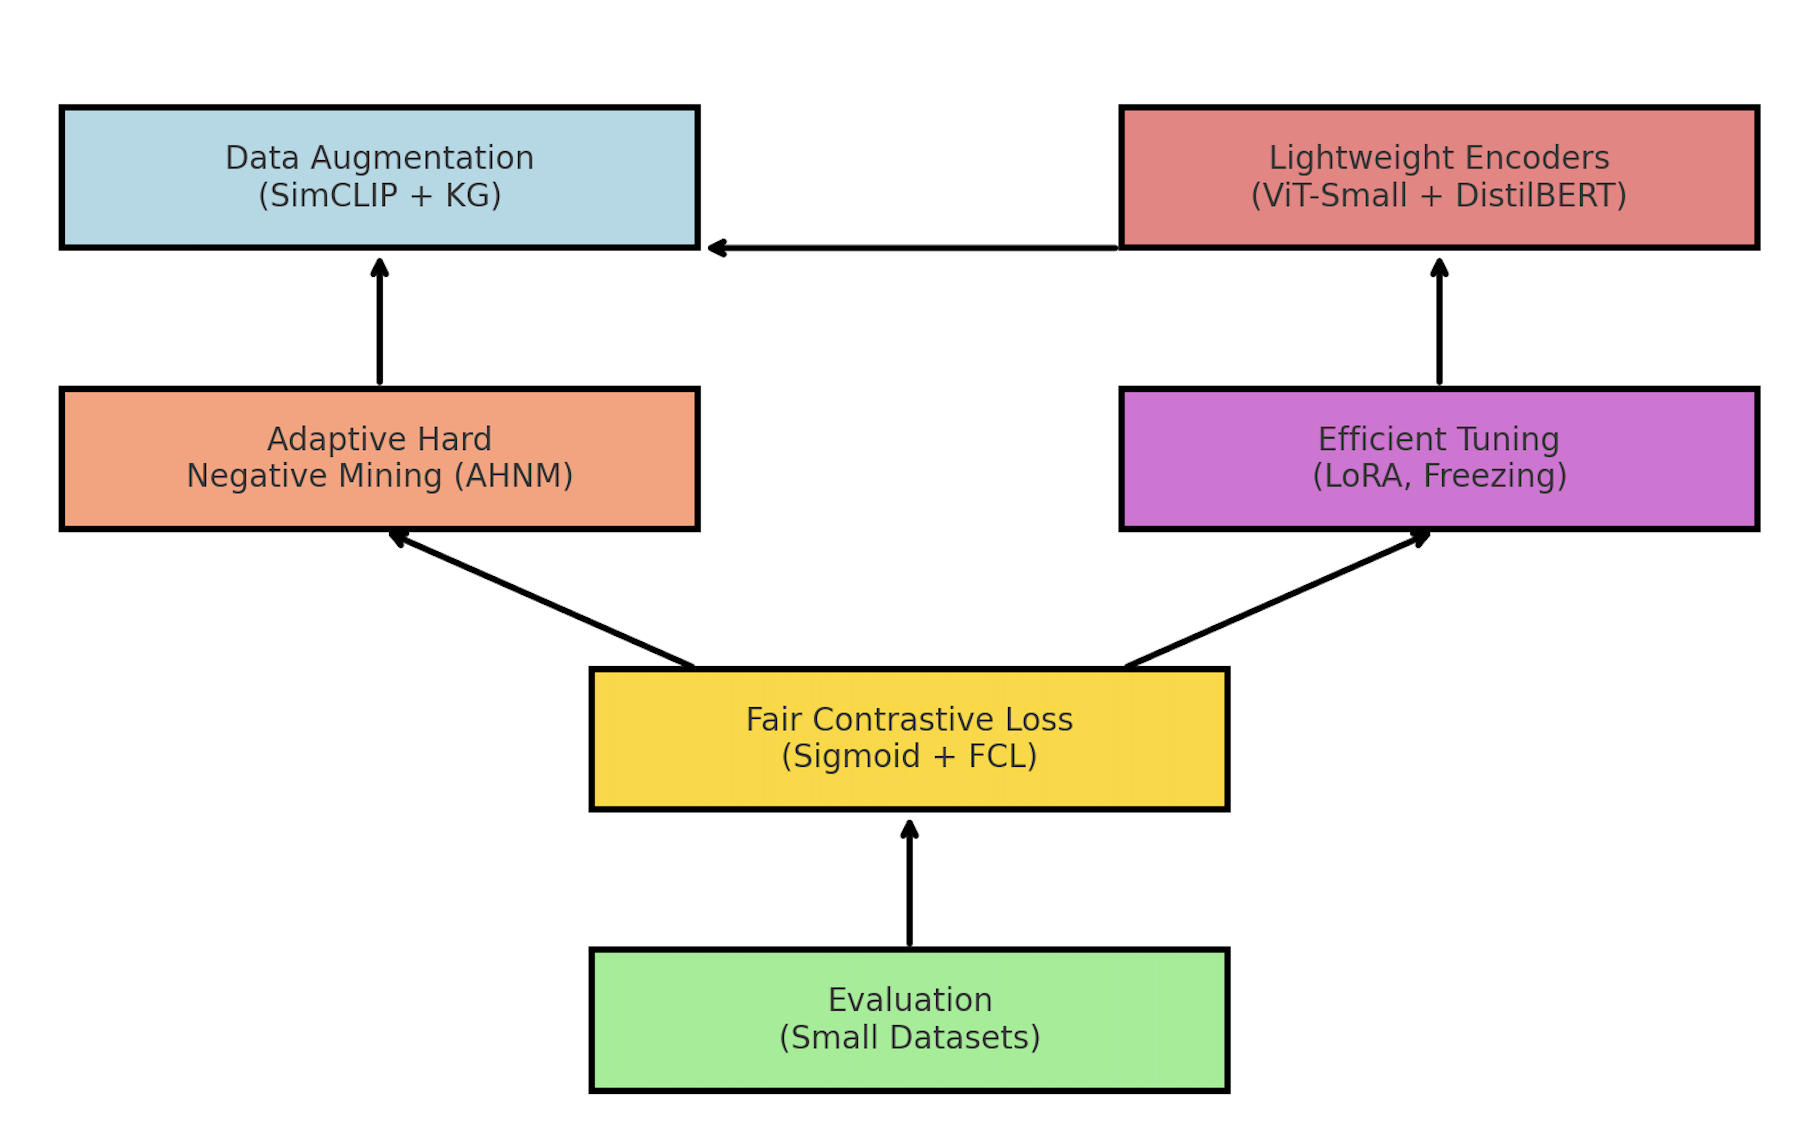
\includegraphics[width=12cm]{proposal/pipeline_draft.png}
    
\end{center}


\printbibliography
\end{document}